\title{Study Guide for Midterm 3}
\author{Dr. Jordan Hanson - Whittier College Dept. of Physics and Astronomy}
\date{\today}
\documentclass[10pt]{article}
\usepackage[a4paper, total={18cm, 27cm}]{geometry}
\usepackage{outlines}
\usepackage{graphicx}
\begin{document}
\maketitle

\section{Memory Bank}

\begin{enumerate}
\item $\vec{F} = q\vec{v} \times \vec{B}$ ... The Lorentz force on a charge $q$ with velocity $\vec{v}$ in a magnetic field $\vec{B}$.
\item $\vec{F} = I\vec{L} \times \vec{B}$ ... The Lorentz force on a conductor of length $\vec{L}$ carrying a current $I$ in a magnetic field $\vec{B}$.
\item $B = \mu_0 I/(2\pi R)$ ... Amp\`{e}re's Law for the B-field a distance $R$ away from a current $I$.
\item $\epsilon = -N \Delta \phi/\Delta t$ ... Faraday's Law.
\item $\phi = \vec{B} \cdot \vec{A}$ ... Definition of magnetic flux.
\item Faraday's Law using \textbf{Inductance}, M: $emf = -M \frac{\Delta I}{\Delta t}$.
\item Typically, we refer to \textit{mutual inductance} between two objects as $M$, and \textit{self inductance} as $L$.  Self-inductance: $\Delta V = -L (\Delta I/\Delta t)$.
\item Units of inductance: V s A$^{-1}$, which is called a Henry, or H.
\item $\epsilon(t) = N B A \omega \cos(\omega t)$ ...  AC voltage from a generator with effective area $A$, B-field $B$, number of turns $N$, and angular frequency $\omega$.
\end{enumerate}

\clearpage

\section{Chapter 11: Magnetic Forces and Fields}

\begin{figure}
\centering
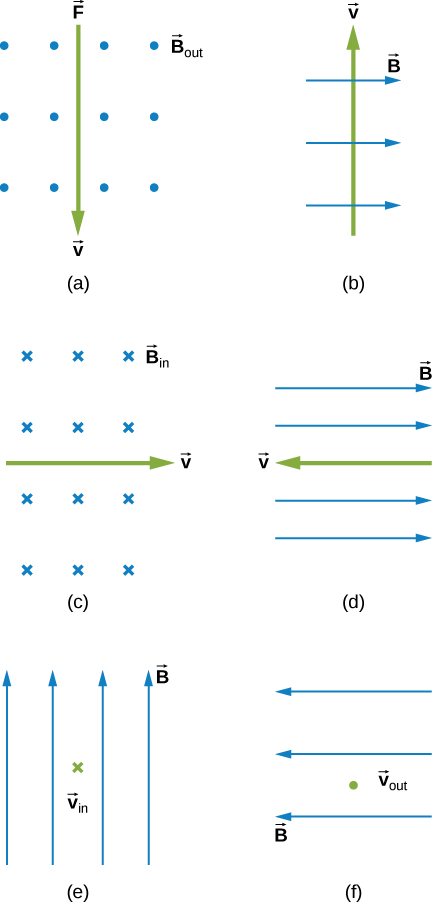
\includegraphics[width=0.25\textwidth]{lorentzDir.jpeg} \hspace{0.5cm}
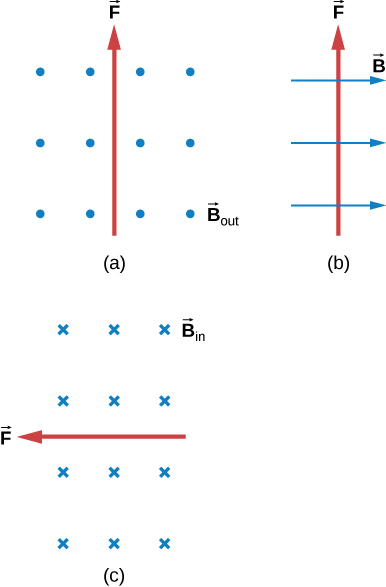
\includegraphics[width=0.3\textwidth]{lorentzDirCurrent.jpeg}
\caption{\label{fig:chap11_1} (Left) A charge $q$ experiences a force $F$ in a B-field. (Right) A current $I$ experiences a force $F$ in B-field.}
\end{figure}

\begin{enumerate}
\item Consider Fig. \ref{fig:chap11_1}.  In each of the cases, determine the direction of the charge or current. \\ \vspace{1cm}
\item Consider Fig. \ref{fig:chap11_2} (right). The cross-sectional dimensions of the copper strip shown are 2.0 cm by 2.0 mm. The strip carries a current of 100 A, and it is placed in a magnetic field of magnitude B = 1.5 T. What are the value and polarity of the Hall potential in the copper strip? \\ \vspace{2cm}
\item Consider Fig. \ref{fig:chap11_2} (left). (a) A 200-turn circular loop of radius 50.0 cm is vertical, with its axis on an east-west line. A current of 100 A circulates clockwise in the loop when viewed from the east. Earth’s field here is due north, parallel to the ground, with a strength of $3 \times 10^{-5}$ T.  What are the direction and magnitude of the torque on the loop? (b) Does this device have any practical applications as a motor? \\ \vspace{1cm}
\end{enumerate}

\begin{figure}[hb]
\centering
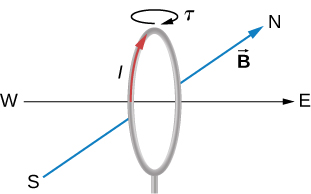
\includegraphics[width=0.3\textwidth]{torqueLoop.jpeg} \hspace{1cm}
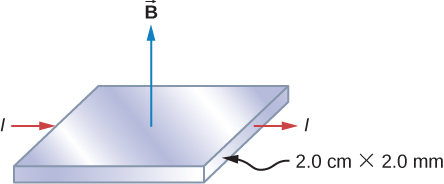
\includegraphics[width=0.4\textwidth]{hallEffect1.jpeg}
\caption{\label{fig:chap11_2} (Left) A charge $q$ experiences a force $F$ in a B-field. (Right) A current $I$ experiences a force $F$ in B-field.}
\end{figure}

\section{Chapter 12: Sources of Magnetic Fields}

\begin{figure}[ht]
\centering
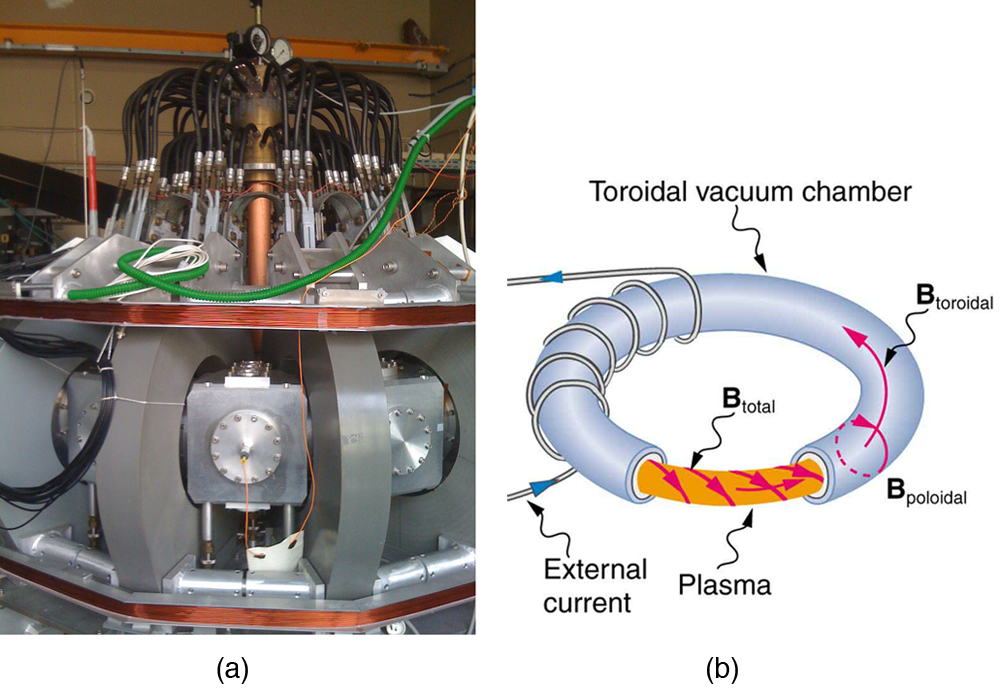
\includegraphics[width=0.35\textwidth,trim=8.5cm 1cm 0cm 3cm,clip=true]{toroid.jpeg}
\caption{\label{fig:chap12_1} A basic diagram of a \textit{toroid}, which is a solenoid wrapped into a circular tube.}
\end{figure}

\begin{enumerate}
\item (a) Using Amp\`{e}re's Law, show that the B-field of a solenoid with $n$ turns per unit length carrying a current $I$ is $B = \mu_0 n I$. (b) What is the B-field inside a solenoid with 1000 turns per meter, carrying a current of 0.1 A? \\ \vspace{1cm}
\item Consider Fig. \ref{fig:chap12_1}.  Suppose the current is 8 Amps, and the number of total turns is 20,000. If the radius of the toroid 5 meters, what is the \textit{toroidal} B-field inside of it? \\ \vspace{1cm}
\item Suppose plasma is trapped inside the toroid, and has an effective current of 0.1 Amp. What is the \textit{poloidal} field (Fig. \ref{fig:chap12_1}) that results from this current, at a distance of 0.5 m from the center of the plasma? \\ \vspace{1cm}
\end{enumerate}

\section{Chapter 13: Electromagnetic Induction}

\begin{figure}
\centering
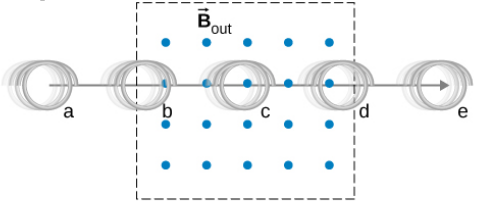
\includegraphics[width=0.33\textwidth]{magdamp.png} \hspace{0.5cm}
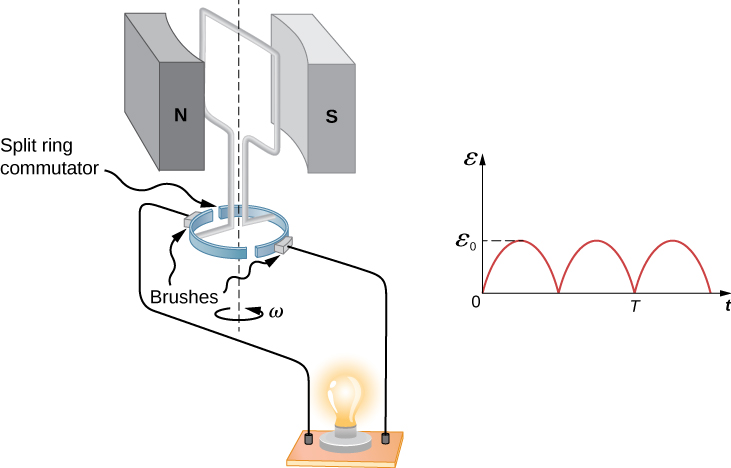
\includegraphics[width=0.33\textwidth]{gen1.jpeg} 
\caption{\label{fig:chap13_1} (Left) \textit{Magnetic damping} occurs when this loop moves through the uniform B-field. (Right) A schematic for an AC generator with commutator brushes.}
\end{figure}

\begin{enumerate}
\item A coil is moved through a magnetic field as shown in Fig. \ref{fig:chap13_1}. The field is uniform inside the rectangle and zero outside. What is the direction of the induced current (if one exists) and what is the direction of the magnetic force on the coil (if there is one) at each position shown?
\begin{itemize}
\item A: Current:$\rule{2cm}{0.15mm}$Force:$\rule{2cm}{0.15mm}$
\item B: Current:$\rule{2cm}{0.15mm}$Force:$\rule{2cm}{0.15mm}$
\item C: Current:$\rule{2cm}{0.15mm}$Force:$\rule{2cm}{0.15mm}$
\item D: Current:$\rule{2cm}{0.15mm}$Force:$\rule{2cm}{0.15mm}$
\end{itemize}
\item The magnetic field in Fig. \ref{fig:chap13_1} is constant and points to the left.  The N loops are rotated through the field with angular frequency $\omega$, and has an area $A$.  Without the commutator brushes, this would make the generated emf
\begin{equation}
\epsilon(t) = N B A \omega \cos(\omega t)
\end{equation}
(a) Explain why the \textit{commutator brushes} make the graph of $\epsilon(t)$ look like the right side of Fig. \ref{fig:chap13_1} (right). (b) Suppose $N = 200$, $A = 100$ cm$^2$, $B = 0.1$ T, and $\omega = 2\pi \times 120$ Hz.  What is the peak emf? (c) If the current flowing through the light is 0.4 A, what is the power consumption of the light, given the emf of the generator? \\ \vspace{2cm}
\end{enumerate}

\section{Chapter 14: Inductance}

\begin{enumerate}
\item What is (a) the rate at which the current though a 0.30-H coil is changing if an emf of 0.12 V is induced across the coil?\\ \vspace{1cm}
\item Consider Fig. \ref{fig:chap14_1}. The current shown in part (a) is increasing, whereas that shown in part (b) is decreasing. In each case, determine which end of the inductor is at the higher potential. \\ \vspace{2cm}
\end{enumerate}

\begin{figure}[hb]
\centering
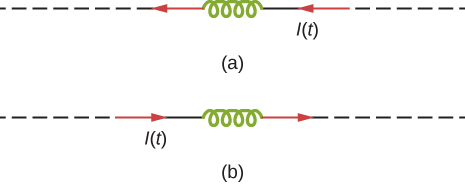
\includegraphics[width=0.5\textwidth]{induct1.jpeg}
\caption{\label{fig:chap14_1} Two inductors of inductance L, and currents $I$ with opposite directions.}
\end{figure}

\end{document}